Anomaly detection systems play a critical role in risk-averse systems by identifying abnormal patterns and adapting to novel expected patterns in data. These systems are particularly vital in the context of Internet of Things (IoT) devices that continuously stream high-fidelity data to control units.

In this rapidly evolving field with long-spanning roots, \citet{Chandola2009} conducted an influential review of prior research efforts across diverse application domains.
Recent studies have underscored the need for holistic and tunable anomaly detection methods accessible to operators \citep{Laptev2015, Kejariwal2015, Cook2020}.

Cook et al. denote substantial aspects that pose challenges to anomaly detection in IoT, including the temporal, spatial, and external context of measurements, multivariate characteristics, noise, and nonstationarity \citep{Cook2020}. To address these complexity issues, \citet{ZHANG2024121506} have successfully employed spatially distributed sensors and time-relative modulation. Their approach has proven effective, particularly in the context of complex non-linear systems, offering potential solutions to some of the challenges posed by IoT data. Huang et al., on the other hand, tackled the problems of detecting global outliers, local outliers, and outlier clusters simultaneously. Their proposed approach, based on density estimation, relies on the notion that density distributions should exhibit minimal variations in local areas. To achieve this, they introduce a novel turning ratio metric, which reduces reliance on hyperparameters and enhances anomaly detection \citep{HUANG2023120799}.

Additionally, feature engineering techniques play a crucial role in capturing contextual properties and enhancing anomaly detection performance \citep{Fan2019}. However, it is worth noting that feature engineering may introduce categorical variables and significantly increase the dimensionality of the data, requiring specific methods for handling large data, sizeable data storage, and substantial computational resources \citep{Talagala2021}. Recently, Li et al. introduced an attribute-weighted outlier detection algorithm, designed for high-dimensional datasets with mixtures of categorical and numerical data. Their approach assigns different weights to individual attributes based on their importance in anomaly detection and uses these weights to calculate distances between data points. Notably, Li et al. demonstrated the superior performance of their algorithm compared to state-of-the-art methods \citep{LI2024121304}. Another strategy for handling high-dimensional data involves using deep learning methods with synthetic normal data to enhance the detection of outliers with subtle deviations, as proposed in \citet{DU2024121161}.

Nevertheless, the presence of nonstationarity, often stemming from concept drift (a shift in data patterns due to changes in statistical distribution) and change points (permanent alterations in system state), presents a substantial challenge \citep{Salehi2018}. In practical scenarios, those changes tend to be unpredictable in both their spatial and temporal aspects. Consequently, they require systems with solid outlier rejection capabilities of intelligent tracking algorithms \citep{Barbosa2019162}. This underscores the critical importance of an anomaly detection method's ability to adapt to evolving data structures, especially in long-term deployments. Nevertheless, as \citep{Tartakovsky2013} remarked, immediate detection is not a feasible option unless there is a high tolerance for false alarms. \added{Promissing balance between early transition detection and low false alarm rate could be achieved by contrastive learning approach. \citet{Deldari2021} have shown that by evaluating cosine similarity between predicted future representation and anticipated representation of time windows, it is possible to detect evolution in data with high accuracy.}

The adaptation of batch models at scale introduces a significant latency in detector adaptation \citep{Wu2021}. Incremental learning methods allowed adaptation while restraining the storage of the whole dataset. The supervised operator-in-the-loop solution offered by \citet{Pannu2012} showed the detector's adaptation to data labeled on the flight.
Others approached the problem as sequential processing of bounded data buffers in univariate signals \citep{Ahmad2017134} and multivariate systems \citep{Bosman201514}.

\subsection{Related Work}
Recent advances in anomaly detection have broadened its scope to include root cause identification governed by the development of explanatory methods capable of diagnosing and tracking faults across the system. Studies can be split into two groups of distinct approaches. The first group approaches explainability as the importance of individual features \citep{Carletti2019, Nguyen2019, Amarasinghe2018}. Those studies allow an explanation of novelty by considering features independently. The second group uses statistical learning creating models explainable via probability. For instance, the integration of variational Bayesian inference probabilistic graph neural network allowed Zhang et al. to model the posterior distribution of sensor dependency for gas leakage localization on unlabeled data \citep{ZHANG2023120542}. Yang et al. recently proposed a Bayesian network (BN) for fault detection and diagnosis. In this BN, individual nodes of the network represent normally distributed variables, whereas the multiple regression model defines weights and relationships. Using the predefined structure of the BN, the authors propose offline training with online detection and diagnosis \citep{Yang2022}.

Given the infrequent occurrence of anomalies and their potential absence in training data, the incorporation of synthetic data or feature extraction for various detected events emerges to assist diagnosis of the system. Brito et al. designed synthetic faults based on expert knowledge and introduced them into a transfer learning classifier to exploit faults in rotating machinery, with a subsequent explanation layer \citep{BRITO2023120860}. Conversely, We et al. leveraged feature selection to expose various types of abnormal behavior. The team presents competitive performance while using change in relationships to provide causal inference \citep{WU2024121539}.

However, it is crucial to underscore that offline training, as previously emphasized, is inherently inadequate when it comes to adapting to anticipated novel patterns, rendering it unsuitable for sustained, long-term operation on IoT devices.

This paper emphasizes the importance of combining adaptability in interpretable anomaly detection and proposes a method that addresses this challenge in real industrial systems. Here we report the discovery and characterization of an adaptive anomaly detection method for existing supervisory control and data acquisition (SCADA) systems, employing streaming IoT data. The ability to diagnose multivariate data while providing root cause isolation via statistical learning, extends our previous contribution to the field as presented in \citep{Wadinger2023}. The proposed algorithm aims to represent a general method that aids a range of existing safety-critical systems where anomaly diagnosis and identification are paramount. The schematic overview of the proposed method's integration is presented in Figure~\ref{fig:overview}.

\begin{figure}[htbp]
    \centering
    \resizebox{\linewidth}{!}{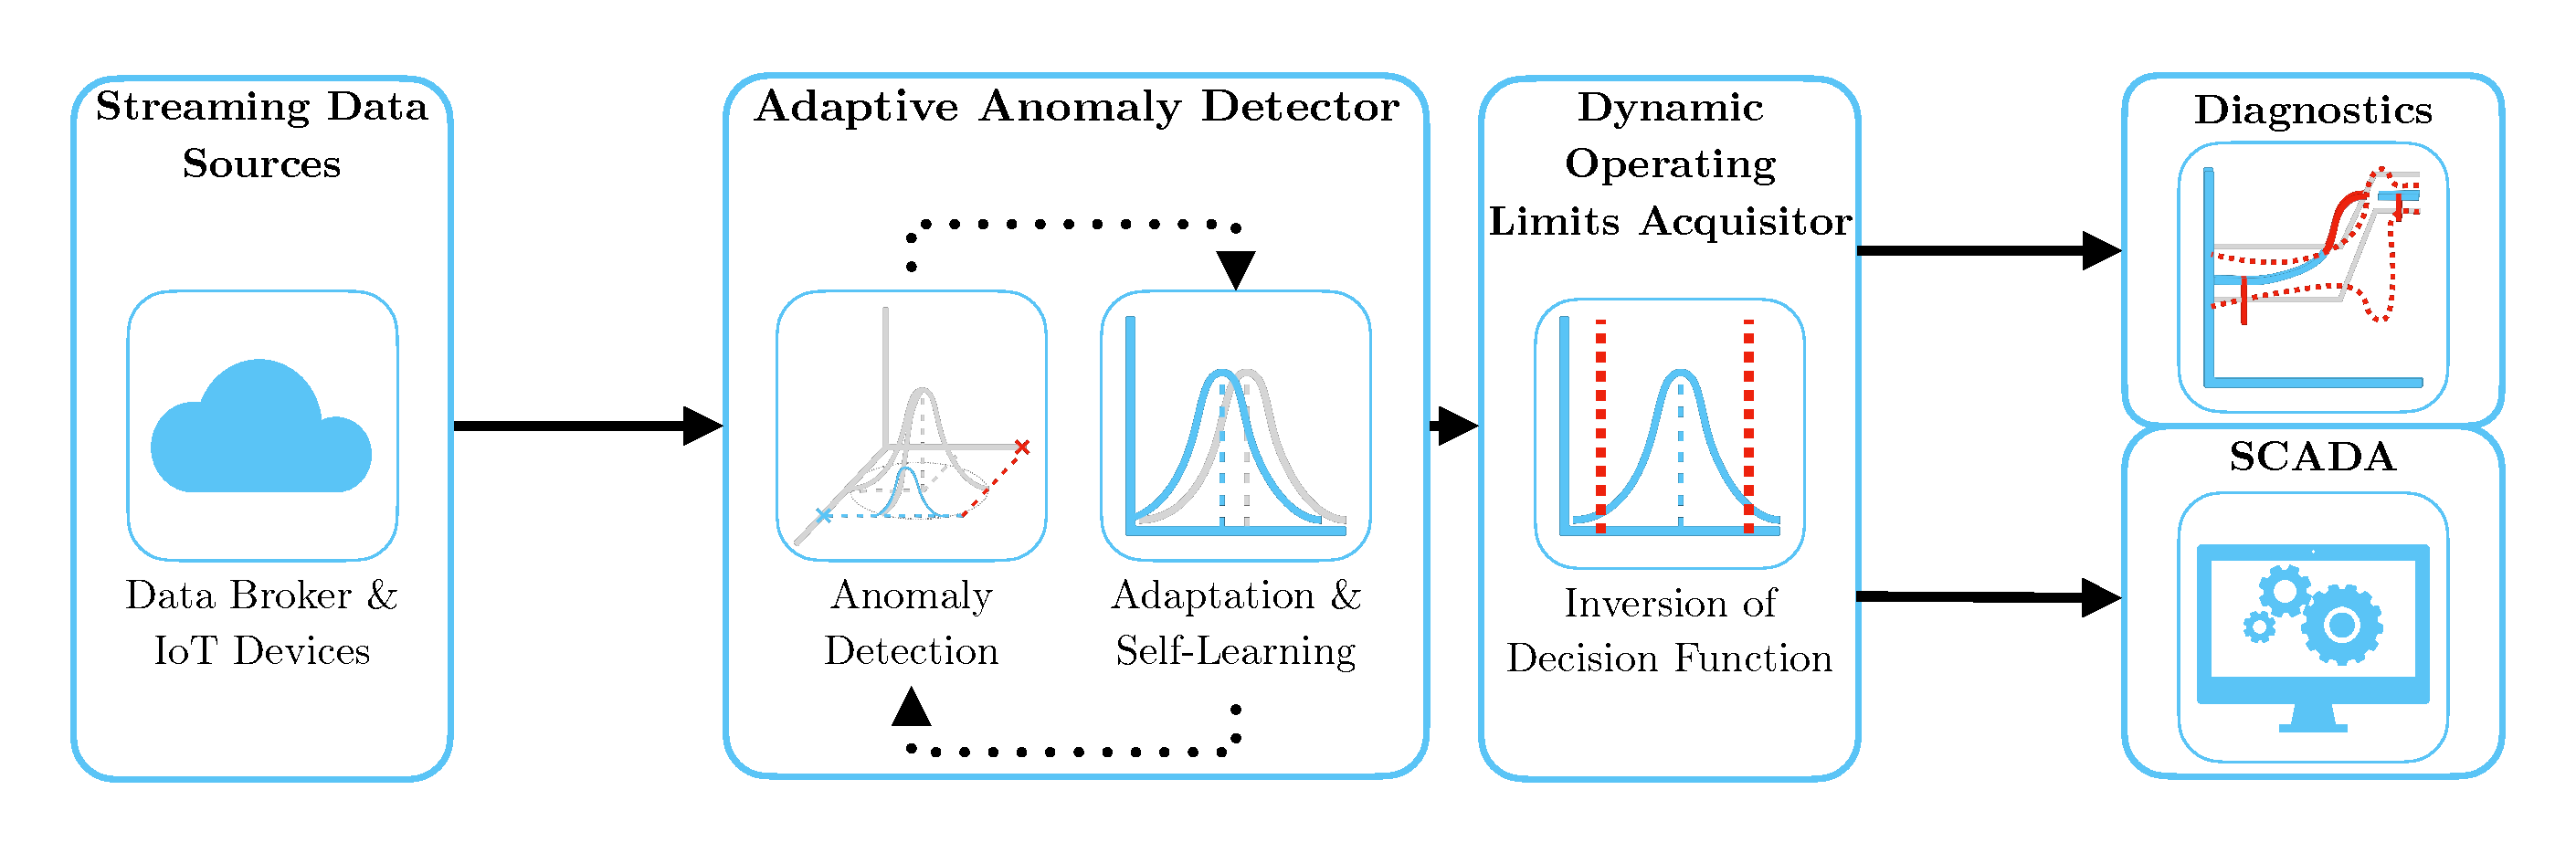
\includegraphics{figures/introduction.pdf}}
    \caption{Schematic representation of the proposed method AID.}
    \label{fig:overview}
\end{figure}

\subsection{Novelty of proposed approach}
The idea of using statistical outlier detection is well-established. We highlight the impactful contributions of Yamanishi et al. in \citep{Yamanishi2002, Yamanishi2004}. The authors propose a method for detecting anomalies in a time series. The method is based on the assumption that the continuous data is generated by a mixture of Gaussian distributions, while discrete data is modeled as histogram density. The authors solve the problem of change point detection as well. However, the adaptation system is unaware of such changes, making the moving window the only source of adaptation. Our self-supervised approach facilitates intelligent adaptation concerning detected change points, to increase the speed of adaptation where the probability of concept drift is high. By leveraging its ability to adapt to changes in operational states, our proposed method operates autonomously when such changes occur. Moreover, \citet{Yamanishi2004} does not attempt to isolate the root cause of the anomaly. Our approach extends statistical outlier detection by incorporating interpretability. This is achieved by evaluating the inverse cumulative distribution function of the latest conditional probabilities for each measurement, considering the remainder of the measurements, and establishing limits that define the threshold for normal event probabilities.

A limited number of studies have focused on adaptation and interpretability within the framework of anomaly detection. Two recent contributions in this area are made by Steenwinckel et al. as reported in \citep{Steenwinckel2018, Steenwinckel2021}. In \citet{Steenwinckel2018}, the authors emphasize the importance of combining prior knowledge with a data-driven approach to achieve interpretability, particularly concerning root cause isolation. They propose a novel approach that involves extracting features based on knowledge graph pattern extraction and integrating them into the anomaly detection mechanism. This graph is subsequently transformed into a matrix, and adaptive region-of-interest extraction is performed using reinforcement learning techniques. To enhance interpretability, a Generative Adversarial Network (GAN) reconstructs a new graphical representation based on selected vectors. However, it is important to note that the validation of this idealized approach is pending further investigation. Lately, \citet{Steenwinckel2021} introduced a comprehensive framework for adaptive anomaly detection and root cause analysis in data streams. While the adaptation process is driven by user feedback, the specific mechanism remains undisclosed. The authors present an interpretation of their method through a user dashboard, featuring visualizations of raw data. This dashboard is capable of distinguishing between track-related problems and train-related issues, based on whether multiple trains at the same geographical location approach the anomaly. Meanwhile, our efforts are directed towards the development of a self-supervised method that can learn autonomously, reducing the reliance on human supervision, which is often constrained by time limitations and can lead to significant delays in adaptation. Our method is distinguished by its straightforward statistical reasoning and the ability to isolate the root cause of anomalies. The interpretability of our method is demonstrated through the establishment of dynamic operating limits for each signal, leveraging conditional probabilities derived from the signal and other system measurements and features. This provides operators with a clear understanding of the system's state and the underlying causes of anomalies and offers interoperability with existing alarm handling mechanisms in SCADA which utilize operating limits.
To the best of our knowledge, this study appears to be one of the initial attempts to introduce a self-supervised approach for adaptive anomaly detection and root cause isolation in SCADA-based systems utilizing IoT data streams.

\subsection{Validation}\label{par:validation}
Two real-world industrial-scale case studies showcase that our proposed method has the capacity to explain anomalies, isolate the root cause, and allow adaptation to change points, allowing long-term deployment at the end users of energy storage systems. We observe similar detection performance, albeit with lower scalability, on benchmark data when comparing our approach to well-established unsupervised anomaly detection methods in streamed data which create a bedrock for many state-of-the-art contributions, such as One-Class SVM \citep{Amer2013, Liu2014, Krawczyk2015, Miao2019, Gozuacik2021}, and Half-Space Trees \citep{Wetzig2019, Lyu2020}.

\subsection{Practical Impact}\label{par:practical_impact}
Potential applications of the proposed method are in the field of energy storage systems, where the ability to detect anomalies and isolate their root causes while adapting to changes in operation and environment, is crucial for the system safety. The proposed method is designed to be integrated into the existing infrastructure of the systems, utilizing IoT data streams on top of well-established SCADA systems. SCADA systems continuously monitor these process data in real-time, embodying alarm handling mechanisms, which are designed to notify operators of the system's abnormal behavior and drive attention to the root of the problem. By comparing the current values to the upper and lower operating limits, they take action when a variable exceeds or falls below these limits. However, safe operating limits are often established based on a combination of equipment design limits and the dynamics of the process \citep{Stauffer2021}. Those are indifferent to the actual state of the system and environmental conditions. The proposed method allows the establishment of dynamic operating limits, based on the current state of the system and its environment, with direct utilization in SCADA systems expecting minimal intervention to existing infrastructure. This allows the system to operate closer or further from its design limits, increasing its safety and profitability. The dynamic operating limits allow operational metrics monitoring, making potential early detection and prevention easier. Using general adaptable methods without interpretability, on the other hand, may pose safety risks and lower total financial benefits, as the triggered false alarms may need to be thoroughly analyzed, resulting in prolonged downtimes.

The main contribution of the proposed solution to the developed body of research is that it:
\begin{itemize}
    \item Interpretable anomaly detector with self-supervised adaptation
    \item Demonstrates interpretability by providing dynamic operating limits
    \item Leverages self-learning approach on streamed IoT data
    \item Utilizes existing SCADA-based industrial infrastruture
    \item Offers faster response time to incidents due to root cause isolation
\end{itemize}

\subsection{Paper Organization}
The rest of the paper is structured as follows: We begin with the problem and motivation in \textbf{Section~\ref{Introduction}}, providing context. Next, in \textbf{Section~\ref{Preliminaries}}, we lay the theoretical groundwork. Our proposed adaptive anomaly detection method is detailed in \textbf{Section~\ref{Proposed Method}}. We then demonstrate real-world industrial-scale applications in \textbf{Section~\ref{Case Study}}. Finally, we conclude the paper in \textbf{Section~\ref{Conclusion}}, summarizing findings and discussing future research directions.
